\subsection{Companion visualization and detailed comparisons}
Figure~\ref{fig:companion} gives the second predetermined case in the same visual format. The following tables retain the detailed ablations, both endpoint controls, kernel frequencies, and protein-only split sensitivity analysis. They use the same completed study outputs as the main comparisons.
\begin{figure}[tbp]
\centering
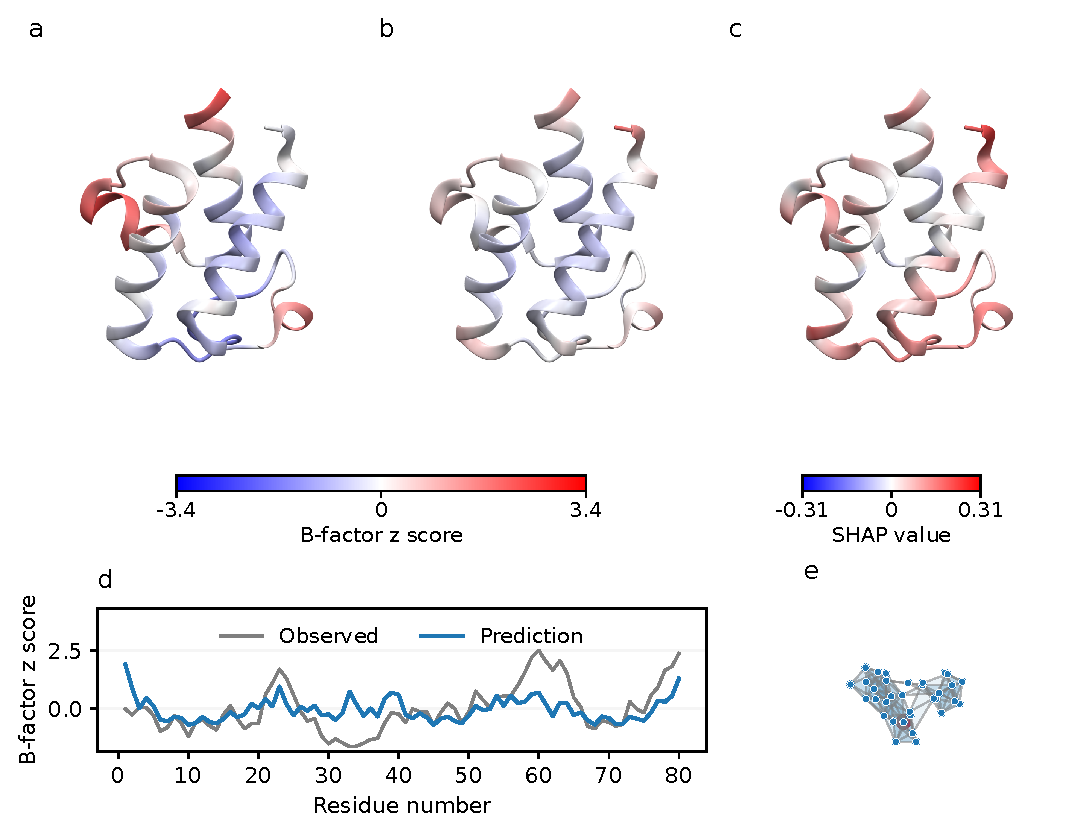
\includegraphics[width=\linewidth]{figures/supp_1X3O.pdf}
\caption{The predetermined companion protein 1X3O. (a,b) Observed within-protein normalized B-factor and the sequence-cluster-held-out graph-plus-center-zero prediction, mapped to the same residue coordinates and shown with a common color scale. (c) The signed sum of TreeSHAP contributions from the 24 center-zero spectral features, in B-factor z-score units. This subtotal excludes graph-feature contributions and the training-background expectation; blue is negative and red positive. (d) Observed and predicted residue profiles provide a direct check alongside the structural views. (e) The local alpha complex at ball radius 4~\AA\ within the fixed 13~\AA\ support of chain A residue 43. The protein, model protocol, and feature grouping were specified before inspecting prediction outcomes.}
\label{fig:companion}
\end{figure}

% Generated by scripts/summarize_study.py; do not transcribe historical metrics here.



\begin{table}[htbp]\centering\small
\caption{Degree-zero ablations of graph plus center-zero features. All models keep all graph features. The paired change is relative to the full multiscale spectral representation.}
\begin{tabular}{lrr}\toprule
Spectral summaries retained & Mean PCC [95\% CI] & Paired change [95\% CI]\\\midrule
Nullities only & 0.627 [0.613, 0.640] & -0.0005 [-0.0029, +0.0018] \\
Positive spectra only & 0.627 [0.613, 0.641] & -0.0000 [-0.0014, +0.0013] \\
Radius 3\,\AA & 0.628 [0.614, 0.641] & +0.0006 [-0.0015, +0.0026] \\
Radius 4\,\AA & 0.625 [0.611, 0.639] & -0.0025 [-0.0045, -0.0006] \\
Radius 5\,\AA & 0.628 [0.614, 0.641] & +0.0006 [-0.0016, +0.0028] \\
Radius 6\,\AA & 0.626 [0.612, 0.640] & -0.0011 [-0.0029, +0.0005] \\
\bottomrule\end{tabular}\end{table}




\begin{table}[htbp]\centering\small
\caption{Persistent-minus-static degree-one comparisons. All additions use twelve features on the same graph-plus-degree-zero baseline. Intervals are paired cluster-bootstrap intervals for mean protein PCC.}
\begin{tabular}{llr}\toprule
Sheaf & Static comparator & Paired PCC change [95\% CI]\\\midrule
Identity & Lower & -0.0004 [-0.0016, +0.0009] \\
Identity & Upper & +0.0000 [-0.0013, +0.0012] \\
Geometric & Lower & +0.0001 [-0.0011, +0.0012] \\
Geometric & Upper & +0.0011 [-0.0005, +0.0029] \\
Center-zero & Lower & +0.0004 [-0.0013, +0.0021] \\
Center-zero & Upper & -0.0005 [-0.0024, +0.0012] \\
\bottomrule\end{tabular}\end{table}




\begin{table}[htbp]\centering\small
\caption{Nonzero degree-one kernel frequencies across all 78,400 residue-centered neighborhoods. Neighborhoods are weighted equally. Identity and geometric nullities agree exactly at all evaluated scales. Equal endpoints describe the corresponding sheaf cohomology; unequal endpoints describe its persistent cohomology restriction rank.}
\begin{tabular}{lrrrr}\toprule
Radius pair (\AA) & \shortstack{Identity\\nonzero (\%)} & \shortstack{Center-zero\\nonzero (\%)} & \shortstack{Mean identity\\nullity} & \shortstack{Mean center\\nullity}\\\midrule
$(3,3)$ & 93.383 & 94.871 & 5.168 & 5.392 \\
$(4,4)$ & 83.679 & 86.844 & 3.102 & 3.488 \\
$(5,5)$ & 34.569 & 43.594 & 0.558 & 0.769 \\
$(6,6)$ & 3.221 & 6.657 & 0.039 & 0.080 \\
$(3,4)$ & 28.578 & 36.213 & 0.360 & 0.481 \\
$(5,6)$ & 0.361 & 2.140 & 0.004 & 0.022 \\
\bottomrule\end{tabular}\end{table}




\begin{table}[htbp]\centering\small
\caption{Protein-only split sensitivity analysis on the same 364 structures.}
\begin{tabular}{lrrr}\toprule
Representation & PCC [95\% CI] & Spearman & RMSE$_z$\\\midrule
Graph geometry & 0.622 [0.608, 0.636] & 0.602 & 0.789 \\
Legacy graph spectra & 0.609 [0.594, 0.623] & 0.598 & 0.848 \\
Graph + legacy spectra & 0.626 [0.612, 0.639] & 0.607 & 0.786 \\
Center-zero spectra & 0.560 [0.543, 0.576] & 0.554 & 0.877 \\
Graph + identity sheaf & 0.625 [0.611, 0.639] & 0.608 & 0.785 \\
Graph + geometric sheaf & 0.626 [0.612, 0.639] & 0.610 & 0.785 \\
Graph + center-zero sheaf & 0.624 [0.610, 0.638] & 0.608 & 0.786 \\
\bottomrule\end{tabular}\end{table}




